%
% fig/pdn-quadrat.tex -- Petr-Douglas-Neumann fuer ein Viereck:
% Aus einem beliebigen Viereck A0=ABCD entsteht in zwei Stufen ein Quadrat.
% Stufe 1: Auf jeder Seite gleichschenklig-rechtwinklige Dreiecke nach aussen
% errichten, Spitzen E,F,G,H bilden A1.
% Stufe 2: Die Mittelpunkte der Seiten von A1 bilden das Quadrat A2.
%
% Beispiel:
%   A=(0,0), B=(6,1), C=(7,5), D=(1,6)
%   E=(3.5,-2.5), F=(8.5,2.5), G=(4.5,8.5), H=(-2.5,3.5)
%   M1=(6,0), M2=(6.5,5.5), M3=(1,6), M4=(0.5,0.5)
%
\begin{figure}
\centering
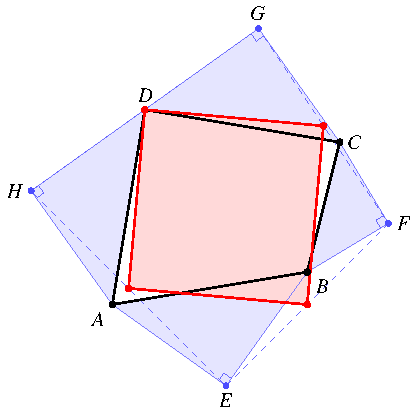
\includegraphics{papers/konstruktion/images/pdn-quadrat.pdf}
\caption{Petr-Douglas-Neumann-Theorem für ein Viereck am Beispiel
$A = 0$, $B = 6 + i$, $C = 7 + 5i$, $D = 1 + 6i$.
Über jeder Seite des Vierecks $ABCD$ (schwarz) wird ein
gleichschenklig-rechtwinkliges Dreieck (rechter Winkel an der Spitze,
markiert) nach aussen errichtet (blau);
die Spitzen $E$, $F$, $G$, $H$ bilden das Viereck $A_1$ (gestrichelt).
Die Mittelpunkte der Seiten von $A_1$ bilden das Quadrat $A_2$ (rot) ---
das Resultat des Verfahrens für $n = 4$.
\label{komplex:figure:pdn-quadrat}}
\end{figure}
